\chapter{SysCo manipulation}
\label{Chap:SysCo}


%-----------------------------------------------------------------------
%-----------------------------------------------------------------------
%-----------------------------------------------------------------------

\section{Introduction}

Coordinate systems (\textbf{SysCo}) types supported by \CdPPP\ are:
\begin{itemize}
\item \textbf{Local}: any Euclidian frame, without any geolocalization or vertical direction knowledge
\item \textbf{GeoC}: geocentric coordinates
\item \textbf{LEuc}: a local Euclidian frame with an affine transformation into geocentric coordinates
\item \textbf{RTL}: a special case of {\tt LEuc}, with the local frame defined by an origin point where Z is normal to ellipsoid and X is on East direction (see ~\ref{SysCoRTL})
\item \textbf{Proj}: any georeferenced system supported by the \href{https://proj.org}{PROJ} library
\end{itemize}

When SysCo is known, its definition is recorded into the file {\tt CurSysCo.xml}, in {\tt Ori} and {\tt PointsMeasure} directories.

%This file can be copied into {\tt MMVII-PhgrProj/SysCo/} with a short name to be used in next commands.
%Example: copy {\tt CurSysCo.xml} as {\tt MMVII-PhgrProj/SysCo/MyCRS.xml}, to be able to use {\tt MyCRS} as a SysCo name.

\section{Setting SysCo}

\subsection{MMVII Commands}
There are several ways to declare a data SysCo:

\begin{itemize}
\item with {\tt SysCo} option in {\tt ImportOri} command that imports orientations into a declared SysCo
\item with {\tt ChSys} option in {\tt ImportGCP} command that declares or transforms ground coordinates on-the-fly
\item some import commands with an implicit SysCo, such as {\tt ImportInitExtSens} that supposes that RPC are always in WGS84 geographical coordinates system in degrees
\item {\tt OriChSysCo} and {\tt GCPChSysCo} commands that transforms orientations and ground points from one SysCo into another
\end{itemize}

\subsection{SysCo definition}
The SysCo definitions for \CdPPP\ commands can be:
\begin{itemize}
\item the name of a file in \CdPPP\ source subfolder {\tt MMVII/MMVII-RessourceDir/SysCo} or in project subfolder {\tt MMVII-PhgrProj/SysCo}, without its extension, only its basename (e.g., {\tt RTL} for MMVII-PhgrProj/SysCo/RTL.xml file)
\item any {\tt PROJ} definition (e.g., {\tt IGNF:LAMB93}, {\tt EPSG:4326} or {\tt '+proj=merc +lat\_ts=56.5 +datum=WGS84'})
\item any string starting with {\tt Local} for a local frame (e.g., {\tt LocalAMRules})
\item {\tt GeoC} for a geocentric frame
\item a string starting with {\tt LEuc}, with the pattern: {\tt LEuc*TX*TY*TZ*Omega*Phi*Kappa}, where the transformation is given in geocentric coordinates, angles in rad
\item a string starting with {\tt RTL}, with the pattern: {\tt RTL*X0*Y0*Z0*Def} (e.g., {\tt RTL*0.675*45.189*0*EPSG:4326}),
where you give the origin point coordinates in a certain PROJ system. Tip: use {\tt SysCoCreateRTL} command to make it automatically (see ~\ref{SysCoRTL})

\end{itemize}


\subsection{Examples}
\begin{itemize}
\item {\tt SysCo=L93} will set the SysCo to Lambert93 (IGNF:LAMB93), as defined in \\
{\tt MMVII/MMVII-RessourceDir/SysCo/L93.xml}
\item {\tt SysCo=IGNF:LAMB1} will set the SysCo to Lambert I
\item {\tt SysCo=LocalPanel} will set the SysCo to a local frame defined as "LocalPanel", that will not be convertible into any other SysCo
\item {\tt SysCo=RTL*0.675*45.189*0*EPSG:4326} will set the SysCo to a tangent local Euclidian frame, with origin ($0.67451979, 45.18899334, 0$) in EPSG:4326
\item {\tt SysCo=GeoC} will set the SysCo to geocentric coordinates
\item {\tt SysCo=AMRealm} will use a project-defined SysCo if {\tt MMVII-PhgrProj/SysCo/AMRealm.xml} exists. If not, "AMRealm" will be used as a PROJ definition, and an error will occur

\end{itemize}


\section{RTL SysCo}
\label{SysCoRTL}

\begin{figure}[h!]
\centering
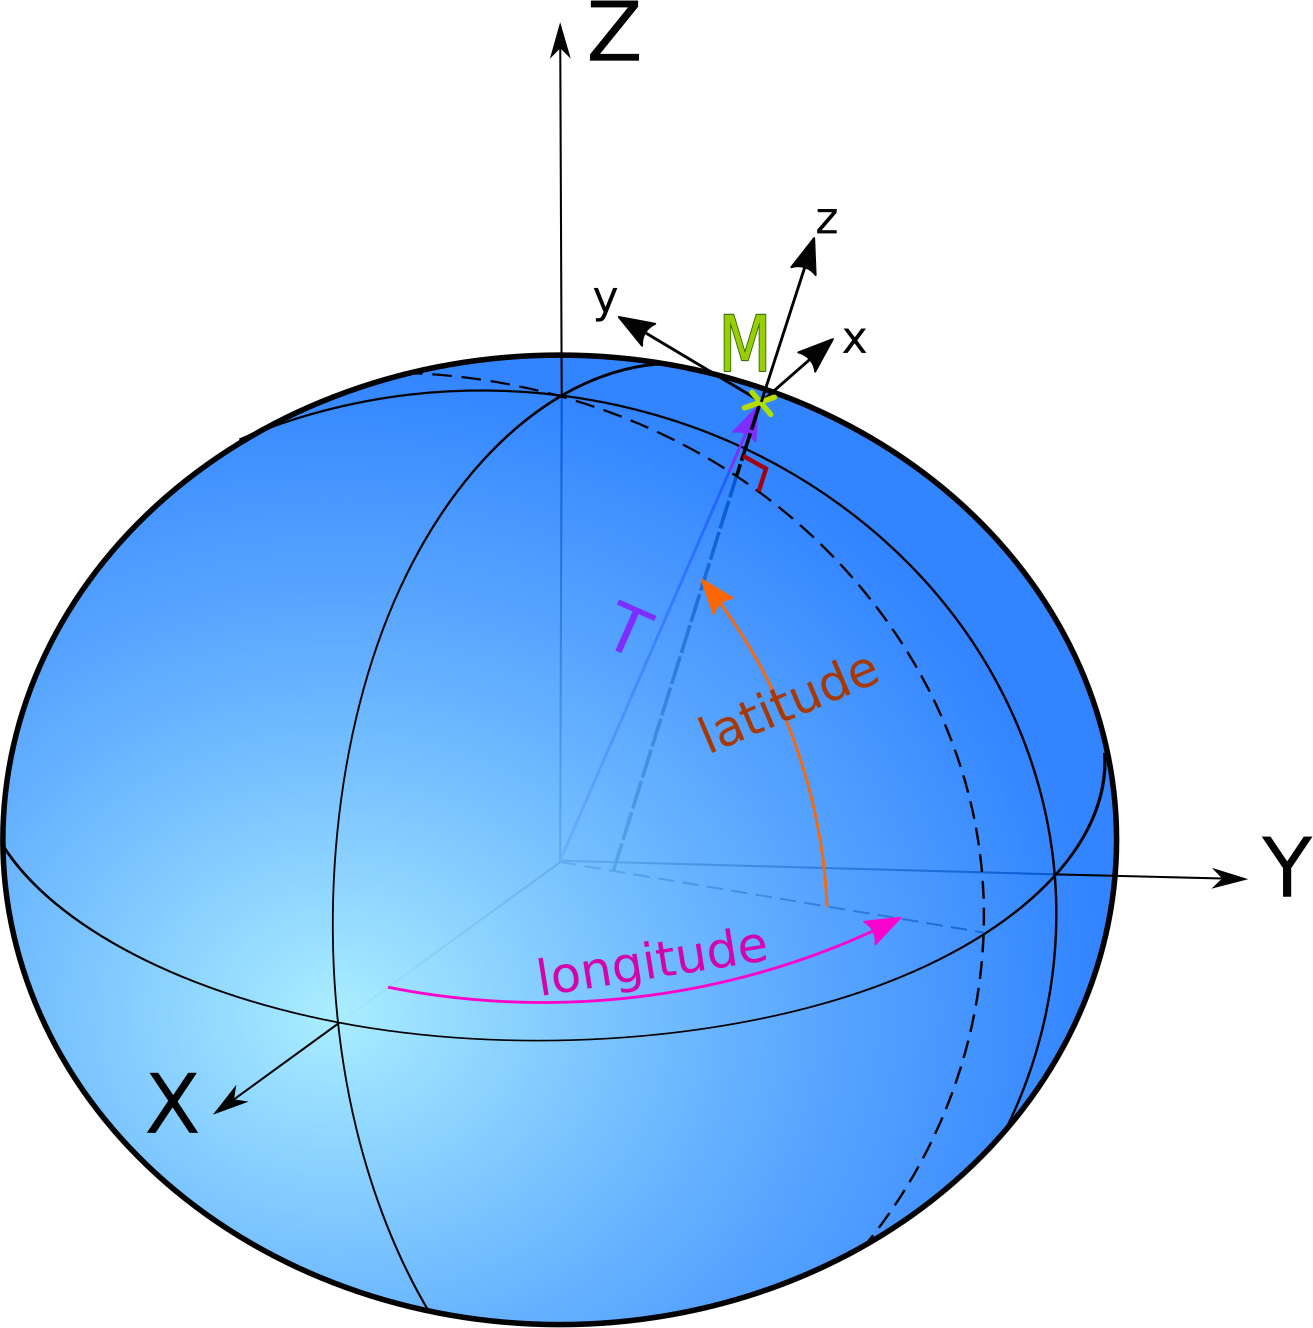
\includegraphics[width=9cm]{CommandReferences/ImagesComRef/cart_geocentr.png}
\caption{Local tangent frame (RTL) SysCo}
\label{fig:RTL}
\end{figure}


\CdPPP\ supposes that the coordinates used during bundle adjustment are Euclidian.

A local tangent frame (RTL) can be defined to simplify ones life. 

{\tt SysCoCreateRTL} command does that from orientations, with the origin point being defined as the average of camera positions or a fixed point.

It creates a file with the chosen name in {MMVII-PhgrProj/SysCo/}.

Then every Ori and GCP is transformed into this RTL frame to be able to keep maximal precision during bundle adjustment.


\section{Testing transformation and PROJ installation}
The {\tt TestProj} command is used to display PROJ log for a transformation between two SysCo.

\begin{verbatim}
 == Mandatory unnamed args : ==
  * string :: Input SysCo definition
  * string :: Output SysCo definition

 == Optional named args : ==
  * [Name=TestPoint] cPtxd<double,3> :: Point in input SysCo to check transformation
\end{verbatim}

Usage example: testing if we can safely convert from ellipsoid height into altitude
(from {\tt IGNF:LAMB93} into {\tt EPSG:5698}, meaning RGF93 v1/Lambert-93 + NGF-IGN69 height):

\begin{verbatim}
MMVII TestProj "L93" "EPSG:5698" TestPoint=[657723,6860710,0]

    PROJ LOG: pj_open_lib(proj.db): call fopen(/usr/share/proj/proj.db) - succeeded
    PROJ LOG: pj_open_lib(proj.ini): call fopen(/usr/share/proj/proj.ini) - succeeded
    Proj "+proj=geocent" to "+proj=latlong" accuracy: 0
    Proj "IGNF:LAMB93" to "+proj=geocent" accuracy: 1
    PROJ LOG: pj_open_lib(proj.db): call fopen(/usr/share/proj/proj.db) - succeeded
    PROJ LOG: pj_open_lib(proj.ini): call fopen(/usr/share/proj/proj.ini) - succeeded
    Proj "+proj=geocent" to "+proj=latlong" accuracy: 0
    PROJ LOG: pj_open_lib(fr_ign_RAF18.tif): call fopen(fr_ign_RAF18.tif) - failed
    PROJ LOG: pj_open_lib(RAF18.gtx): call fopen(RAF18.gtx) - failed
    PROJ LOG: pj_open_lib(fr_ign_RAF20.tif): call fopen(fr_ign_RAF20.tif) - failed
    PROJ LOG: pj_open_lib(fr_2019m.asc): call fopen(fr_2019m.asc) - failed
    PROJ LOG: pj_open_lib(fr_2019z.asc): call fopen(fr_2019z.asc) - failed
    Proj "EPSG:5698" to "+proj=geocent" accuracy: -1
                    SysIn                 =>                 SysOut                
    [657723.00000,6860710.00000,0.00000]  =>  [657723.00000,6860710.00000,-0.00000]
\end{verbatim}

Here, for the {\tt TestPoint}, the output altitude is equal to the height, which in fact should be $-43.77823$.
The PROJ log messages show that the RAF grids are missing, hence the error.

See ~\ref{ProjData} for PROJ additional data installation.


\section{Proj additional data}
\label{ProjData}
Additional data for PROJ can be downloaded here: \url{https://download.osgeo.org/proj/}.

On GNU/Linux, it should be copied into $\sim${\tt /.local/share/proj/}.

On Windows, it should be copied into {\tt MMVII\textbackslash share\textbackslash proj\textbackslash}.



%-----------------------------------------------------------------------
%-----------------------------------------------------------------------
%-----------------------------------------------------------------------

\chapter{Survey compensation (WIP)}
\label{Chap:TopoUser}


\section{Survey introduction}

{\tt MMVII} can add topographic survey measurements in global adjustments.
The following measurements types are currently supported :

\begin{itemize}
    \item distances
    \item pseudo-horizontal angles
    \item pseudo-vertical angles
    \item direct cartesian vector observation
\end{itemize}

These measurements are made from an instrument that can be vertical or not.
For now, the vertical is modeled as the Earth's ellipsoid normal. Vertical deflection grids may be added later.

The measurements can be made between cameras Ori, GCP or new points (that will be inserted into the last GCP set of the adjustment).

Two {\tt MMVII} commands can use survey measurements in compensation:
\begin{itemize}
    \item {\tt OriBundleAdj} via the {\tt TopoFile} option
    \item {\tt TopoAdj} (see below)
\end{itemize}

The topo measurements file can be given as a {\tt MMVII} json or xml topo file, or in a simplified text format (named {\tt obs} file) inherited from IGN's Comp3D compensation software.

The {\tt MMVII} topo files record all the input and output data, organized as the internal {\tt MMVII} objects during compensation.
The {\tt obs} format is simplified and easily human-editable. It is the preferred input format for simple station-based measurements.

All the measurements files must be put in the {\tt MMVII-PhgrProj/Topo/[ObsName]} folder.

\section{{\tt obs} file format}
\label{sec:compObsFormat}
Note: {\tt MMVII} supports only a subset of Comp3D format.

{\tt obs} files are text files with fields delimited by any number of spaces or tabs. Blank lines are overlooked.
The {\tt *} character defines a comment that goes up to the end of the line.

Example:

\begin{verbatim}
    7 St1 Or1   0.0000 0.0010 * horizontal reference
    6 St1 Or1 100.0000 0.0010 * zenithal angle
    3 St1 Or1  20.0000 0.0010 * distance

    5 St1  E1  100.0000 0.0010 * horizontal angle
    6 St1  E1  100.0000 0.0010
    3 St1  E1 1000.0000 0.0010
\end{verbatim}

An observation line is composed by:

\begin{itemize}
    \item code: an integer representing the type of observation (see below)
    \item station name
    \item target name
    \item measurement value (in meters for distances, in gon for angles)
    \item measurement a priori $\sigma$ (in meters for distances, in gon for angles)
    \item anything else is ignored until the end of the line
\end{itemize}

The observations codes are:

\begin{itemize}
    \item 3: 3d distance
    \item 5: local pseudo-horizontal angle
    \item 6: local pseudo-zenithal angle
    \item 14: local X difference
    \item 15: local Y difference
    \item 16: local Z difference
\end{itemize}

All these observations are made in the station frame.

In the previous example, {\tt St1}, {\tt Or1} and {\tt E1} are points name.
They can refer to GCP, cameras or undefined points.

To declare the orientation status of the next station, the following lines have to be
added to the {\tt obs} file (by default stations are supposed vertical/plumb) :

\begin{itemize}
    \item \texttt{\#FIX}: the station vertical and oriented to North
    \item \texttt{\#VERT}: the station vertical, only horizontal orientation is free
    \item \texttt{\#BASC}: the station orientation has 3 degrees of liberty 
\end{itemize}

To distinguish several vertical stations on the same point, the observation code {\tt 7} can be used:

\begin{verbatim}
    7 station target 100 0.001
\end{verbatim}

is equivalent to:

\begin{verbatim}
    #VERT
    5 station target 100 0.001
\end{verbatim}


\section{Survey obs to make minimal external constraints}

For any kind of adjustment, minimal constraints can be useful to get the measurements internal precision.
In general, several GCP with known coordinates are used to fix the frame, but their inconsistency may
impact the computation.

In a 3D adjustment, up to 7 external constraints have to be provided to fix the frame translation, rotation and scale.

With photogrammetry, one camera pose can be fixed to fix 6 external constraints. The scale can then be given with an obs file:
\begin{verbatim}
    * 10 meters between IMG1.JPG and IMG2.JPG poses
    3  IMG1.JPG  IMG2.JPG 10.0000 0.0010   
\end{verbatim}

An other possibility is to constrain the coordinates a one GCP, then add an obs file to fix the scale and the 3 rotations:
\begin{verbatim}
    3  IMG1.JPG  IMG2.JPG 10.0000 0.0010   * scale constraint

    #FIX  * do not add a rotation unknown
    5  IMG1.JPG  GCP_10  0   0.0010   * GCP_10 is north from IMG1.JPG => constraints Rz

    * two Za=Zb constraints between non-aligned points to constrain Rx and Ry
    16  GCP_03  GCP_10  0 0.0010
    16  GCP_03  GCP_11  0 0.0010
    
\end{verbatim}


\section{{\tt TopoAdj} command}

The {\tt TopoAdj} command can perform an adjustment between survey and GCP constraints.
It is used as a substitute to {\tt OriBundleAdj} when there are no cameras.

The GCP folder must then have a RTL CurSysCo.xml file, and do not have to declare all the points
referred to by topo observations, but automatic points initialization is not completed for now.

The SysCo has to be of type RTL, except if there are only distances measurements.

\begin{verbatim}
   For command : TopoAdj 
   => Topo adjustment
   => Srce code entry in :/home/JMMuller/micmac/MMVII/src/BundleAdjustment/cAppliTopoAdj.cpp

 == Mandatory unnamed args : ==
  * string [Topo,In] :: Dir for Topo measures
  * string [Topo,Out] :: Dir for Topo measures output
  * string [PointsMeasure,In] :: Dir for points initial coordinates
  * string [PointsMeasure,Out] :: Dir for points final coordinates

 == Optional named args : ==
  * [Name=GCPW] double :: Constrained GCP weight factor (default: 1)
  * [Name=DataDir] string :: Default data directories  ,[Default=Std]
  * [Name=NbIter] int :: Number of iterations ,[Default=10]
  * [Name=GCPFilter] string :: Pattern to filter GCP by name
  * [Name=GCPFilterAdd] string :: Pattern to filter GCP by additional info
  * [Name=GCPDirOut] string [PointsMeasure,Out] :: Dir for output GCP
  * [Name=LVM] double :: Levenberg–Marquardt parameter (to have better conditionning of least squares) ,[Default=0]

\end{verbatim}



\section{\texttt{TopoComp} Bench first example}
\label{subsec:topoBench}

The example is created by the method \texttt{cTopoData::createEx1()}.
We will describe the input files equivalent for the \texttt{TopoAdj} command.


\subsection{Creating the points}

The points are declared, their initial coordinates and the sigmas on their coordinates constraints
are given in a GCP file. 

3 points have coordinates constraints at 1cm ($A$, $B$, $C$). They form an isosceles triangle
on an horizontal plane.
A 4th point ($D$) is declared above the other. It has no {\tt \_\_Opt\_\_Sigma2} attribute as this point is free.
(Fig. \ref{fig:topoEx1}). Note that depending on the initial coordinates for $D$, the computation may no succeed
(e.g. if $A$ and $D$ have the same initial coordinates, the distance formula derivatives are $NaN$).

A {\tt CurSysCo.xml} must come along this GCP file to describe the RTL SysCo.


\begin{figure}[!h]
\centering
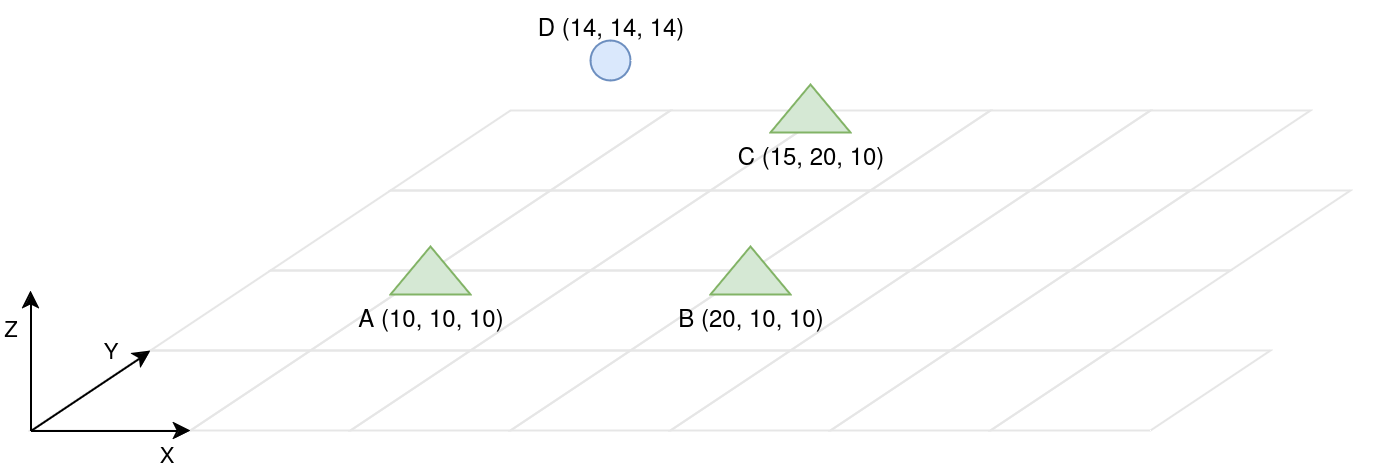
\includegraphics[width=12cm]{Programmer/benchtopo1b.png}
\caption{The 3 fixed points and the free point}
\label{fig:topoEx1}
\end{figure}

The summarized content of the GCP file:

\begin{lstlisting}
      <SetGCP>
         <NameSet>"terrain"</NameSet>
         <Measures>
            <el>
               <Name>"A"</Name>
               <Pt>10 10 10</Pt>
               <AdditionalInfo>""</AdditionalInfo>
               <__Opt__Sigma2>.0001 0 0 .0001 0 .0001</__Opt__Sigma2>
            </el>
            <el>
               <Name>"B"</Name>
               <Pt>20 10 10</Pt>
               <AdditionalInfo>""</AdditionalInfo>
               <__Opt__Sigma2>.0001 0 0 .0001 0 .0001</__Opt__Sigma2>
            </el>
            <el>
               <Name>"C"</Name>
               <Pt>15 20 10</Pt>
               <AdditionalInfo>""</AdditionalInfo>
               <__Opt__Sigma2>.0001 0 0 .0001 0 .0001</__Opt__Sigma2>
            </el>
            <el>
               <Name>"D"</Name>
               <Pt>14 14 14</Pt>
               <AdditionalInfo>""</AdditionalInfo>
            </el>
         </Measures>
      </SetGCP>
\end{lstlisting}


\subsection{Creating the observations}

The distances from $D$ to $A$, $B$ and $C$
are measured. For redundancy and error evaluation, the distance from $D$ to $C$ is measured twice
with different values (Fig. \ref{fig:topoEx2}).

\begin{figure}[!h]
\centering
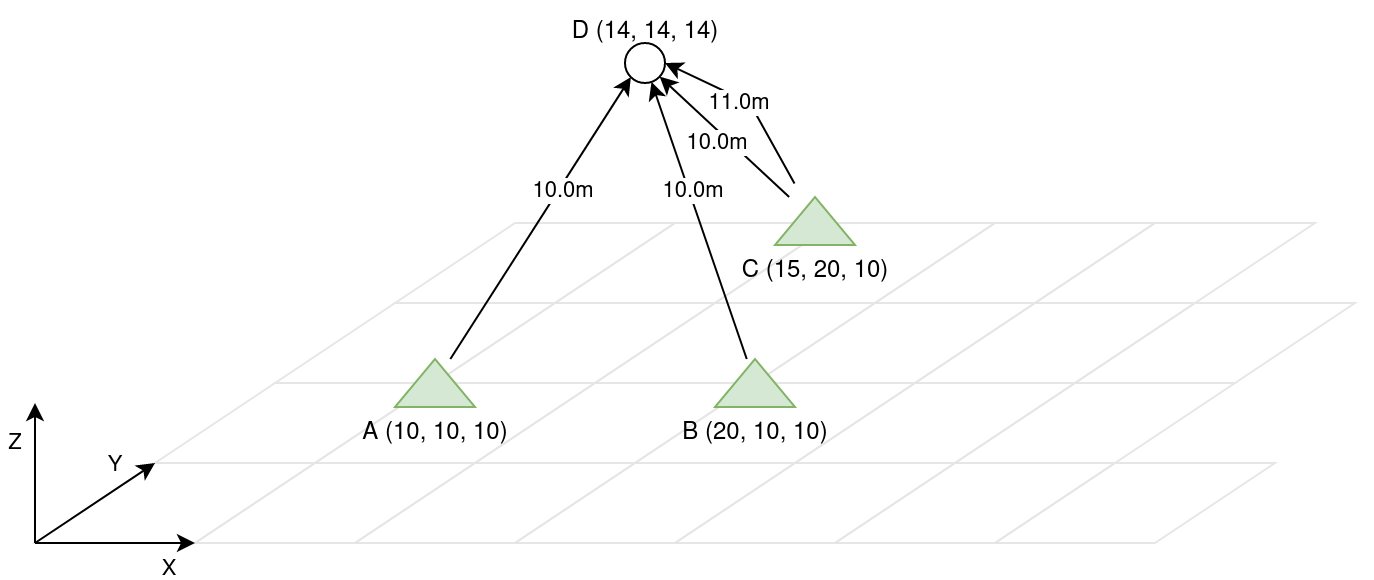
\includegraphics[width=12cm]{Programmer/benchtopo2.png}
\caption{Point $D$ is determined by measured distances}
\label{fig:topoEx2}
\end{figure}

Observations are represented in an {\tt obs} file:
\begin{lstlisting}
    3  D  A  10.0  0.1
    3  D  B  10.0  0.1
    3  D  C  10.0  0.1
    3  D  C  10.1  0.1
\end{lstlisting}

Here a implicit station is created, based on point D.
As no orientation status is given, the station is supposed verticalized.
It should have an horizontal orientation degree of liberty.
But since there is no observations able to determine the station orientation,
it is automatically set as fixed (as if a {\tt \#FIX} line was added at the start of the file).

\subsection{Outputs}

After a computation, the output GCP file contains the final coordinates of every point, including
points that were not declared in the input GCP, but referenced in the survey measurements.

The output Topo file contains info about all the stations and observations,
with output values as residuals:

\begin{lstlisting}
<TopoData>
 <AllObsSetStations>
    <el>
       <TopoObsSetData>
          <Type>"Station"</Type>
          <AllObs>
             <el>
                <TopoObsData>
                   <Type>"Dist"</Type>
                   <Pts>    <el>"D"</el>     <el>"A"</el>       </Pts>
                   <Measures>    <el>10</el>      </Measures>
                   <Sigmas>   <el>0.1</el>     </Sigmas>
                   <__Opt__LastResiduals>  <el>-0.000000000000002</el>  </__Opt__LastResiduals>
                </TopoObsData>
             </el>
[...]
             <el>
                <TopoObsData>
                   <Type>"Dist"</Type>
                   <Pts>      <el>"D"</el>     <el>"C"</el>          </Pts>
                   <Measures>     <el>10.1</el>         </Measures>
                   <Sigmas>       <el>0.1</el>           </Sigmas>
                   <__Opt__LastResiduals>  <el>-0.050000000000001</el>  </__Opt__LastResiduals>
                </TopoObsData>
             </el>
          </AllObs>
          <StationOriStatus>"#FIX"</StationOriStatus>
          <__Opt__Out_G0>0</__Opt__Out_G0>
       </TopoObsSetData>
    </el>
 </AllObsSetStations>
</TopoData>
\end{lstlisting}

This Topo file can be used as input for an other adjustment (it is completely equivalent to the {\tt obs} file).
